\documentclass[tikz, border=10pt]{standalone}
\usetikzlibrary{shapes.geometric, positioning}
\begin{document}
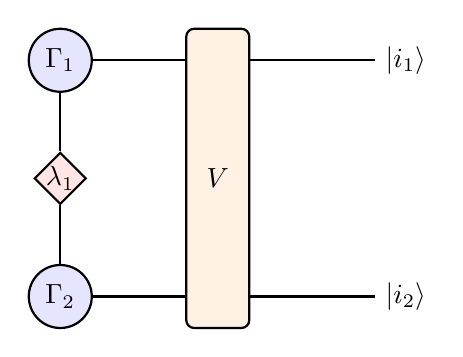
\begin{tikzpicture}[
    thick,
    gamma/.style={circle, draw=black, minimum size=8mm, fill=blue!10, inner sep=0pt},
    lambda/.style={diamond, draw=black, minimum size=6mm, fill=red!10, inner sep=0pt},
    gate1/.style={rectangle, draw=black, minimum size=8mm, fill=green!10, rounded corners=1mm},
    gate2/.style={rectangle, draw=black, minimum width=8mm, minimum height=3.8cm, fill=orange!10, rounded corners=1mm},
    wire/.style={draw, thick}
]

% --- Начальное состояние (t=0) ---
\node[gamma] (G1) at (0, 0) {$\Gamma_{1}$};
\node[lambda] (L1) at (0, -1.5) {$\lambda_{1}$};
\node[gamma] (G2) at (0, -3) {$\Gamma_{2}$};

% Вертикальные связи
\draw[wire] (G1) -- (L1) -- (G2);

% --- Гейт V на [1, 2] (t=1) ---
\node[gate2] (V_1_1_2) at (2, -1.5) {$V$};
\draw[wire] (0, 0 -| G1.east) -- (0, 0 -| V_1_1_2.west);
\draw[wire] (0, -3 -| G2.east) -- (0, -3 -| V_1_1_2.west);

% --- Открытые индексы (выходы) ---
\coordinate (out1) at (4, 0);
\draw[wire] (0, 0 -| V_1_1_2.east) -- (out1);
\node[right] at (out1) {$|i_{1}\rangle$};
\coordinate (out2) at (4, -3);
\draw[wire] (0, -3 -| V_1_1_2.east) -- (out2);
\node[right] at (out2) {$|i_{2}\rangle$};
\end{tikzpicture}
\end{document}